\section{Why product differentiation matters}\label{sec:04-why}

This section explains why differentiation is the normal case, which economic questions it raises, and how theory
and empirical work divide the resulting problem between them.

\subsection{Differentiation is the rule}\label{sec:04-why-rule}

Products are \emph{differentiated} when consumers do not regard them as perfect substitutes. Products differ in
physical characteristics (horsepower, sugar content, screen size) and in location (a gasoline station on one
corner or the next). They also differ in brand and reputation, in the service that comes with them, and in timing
(a morning or an evening flight). Two consumers facing the same prices often buy different products. The same consumer may switch
products when relative prices change, but not all of her demand moves at once.

Differentiation appears even in markets that look homogeneous. A branded drug and its generic version are
chemically identical, yet the branded version keeps a large share at a much higher price. Gasoline is a
standardized commodity, yet stations differ in location, brand and amenities, and nearby stations compete far
more intensely than distant ones. Near-homogeneous markets exist, but they are rare. Wholesale electricity and
refined sugar are two examples, and they are the settings of \citet{Wolfram1999} and
\citet{GenesoveMullin1998}, studied in \cref{ch:conduct}.

Differentiation changes the objects that describe a market. Let $q_j(p)$ be the demand for product $j$ as a
function of the whole price vector $p = (p_1, \dots, p_J)^\top$. Three consequences follow.
\begin{enumerate}[label=(\roman*)]
  \item There is no single market price. There is a vector of prices, one for each product, and these prices can
  differ persistently.
  \item There is no natural boundary of the market. Every product substitutes for many others to some degree, so
  the set of ``competitors'' is a matter of degree.
  \item The own-price elasticity of product $j$,
  \begin{equation*}
  \varepsilon_j(p) = -\frac{\partial q_j(p)}{\partial p_j}\frac{p_j}{q_j(p)},
  \end{equation*}
  depends on rivals' prices and on how close rival products are in the eyes of consumers. Market power is no
  longer summarized by one elasticity. It depends on the whole matrix of own and cross effects.
\end{enumerate}
Differentiation also resolves a puzzle from \cref{ch:theory}. With a homogeneous good, two price-setting firms
with equal constant costs drive price down to marginal cost (\cref{prop:02-bertrand}). The reason is that a
small price cut captures the whole market, so demand is discontinuous in prices. With differentiated products a
small price cut attracts only the marginal consumers, demand is continuous, and price competition among a few
firms leaves positive margins.

\subsection{Questions that require a demand system}\label{sec:04-why-questions}

A \emph{demand system} is the vector of demand functions $q(p, z) = (q_1(p, z), \dots, q_J(p, z))^\top$ for all
$J$ products, as functions of all prices $p$ and of demand shifters $z$ (characteristics, income, season). Many
central questions of industrial organization cannot be answered without one. \Cref{tab:04-questions} lists five
of them with the object each requires. We discuss each in turn.

\begin{table}[htbp]
\centering
\caption{Questions about differentiated-product markets and the demand objects they require}
\label{tab:04-questions}
\footnotesize
\begin{tabularx}{\textwidth}{@{}>{\raggedright\arraybackslash}p{3.3cm}X>{\raggedright\arraybackslash}p{2.6cm}@{}}
\toprule
Question & Demand object required & Treated in \\
\midrule
Measuring market power & Own and cross price derivatives at observed prices, plus a model of price setting
& \cref{sec:04-bertrand,sec:04-supply} \\[2pt]
Welfare effects of mergers & Diversion between the merging products and their margins, or the full system for
simulation & \cref{sec:04-diversion}, \cref{ch:mergers} \\[2pt]
Effects of taxes and tariffs & Pass-through, which depends on second derivatives of demand and on strategic
responses & \cref{prop:04-passthrough}, \cref{ch:theory} \\[2pt]
Product introduction and positioning & Demand for products not yet sold, so tastes over characteristics &
\cref{sec:04-spaces,sec:04-location} \\[2pt]
Welfare from new goods and price indices & Demand far from observed prices, up to the price at which demand for
the new good is zero & \cref{ch:newgoods} \\
\bottomrule
\end{tabularx}
\end{table}

\casehead{Measuring market power}
Accounting data rarely measure marginal cost (\cref{ch:intro}). The approach of the New Empirical Industrial
Organization \citep{Bresnahan1989} infers markups from behavior instead. With differentiated products this
requires the own and cross price derivatives of demand at observed prices and a model of how firms set prices.
Given both, \cref{sec:04-bertrand-matrix} shows that markups follow from a matrix inversion, and
\cref{sec:04-supply} turns them into estimates of marginal cost.

\casehead{Mergers}
A merger of two sellers of substitutes raises prices when the merged firm internalizes the sales that each product
loses to the other. The size of this effect depends on the share of one product's lost customers who would switch
to the other, a quantity called the diversion ratio (\cref{sec:04-diversion}). It also depends on the margins
earned on those customers. Predicting post-merger prices requires the full demand system and a model of supply
(\cref{sec:04-counterfactuals}, \cref{ch:mergers}).

\casehead{Taxes and tariffs}
The incidence of a tax or tariff depends on how much of a cost increase firms pass on to prices. In
\cref{ch:theory} pass-through depends on the curvature of demand. With differentiated products it also depends on
how rivals respond to one another's price changes. This requires second derivatives of the demand system
(\cref{prop:04-passthrough}).

\casehead{Product introduction}
Whether a firm should launch a new product depends on how many sales the product takes from rivals and how many it
takes from the firm's own products. Answering this before launch requires a model that predicts demand for a
product nobody has bought yet. This pushes us toward demand defined over product characteristics
(\cref{sec:04-spaces}) and toward models of product choice (\cref{sec:04-location}).

\casehead{New goods and price indices}
A consumer price index that ignores new goods overstates the increase in the cost of living. Valuing a new good
requires the price at which its demand would be zero, the \emph{virtual price}, and the area under the demand
curve above the observed price. \citet{Hausman1997} computes it for a new breakfast cereal from an estimated
demand system (\cref{ch:newgoods}). The calculation extrapolates demand far from observed prices, so it depends
heavily on functional form.

\subsection{Demand systems and market definition}\label{sec:04-why-market}

In a homogeneous-good industry the market is the set of sellers of the identical good, and concentration
measures such as the Herfindahl index $\HHI = \sum_i s_i^2$ are computed on it (\cref{ch:intro},
\cref{sec:02-concentration}). With differentiated products this boundary does not exist, yet antitrust practice
still needs one. Agencies and courts draw it with the \emph{hypothetical monopolist test}. Imagine a
profit-maximizing firm that owned every product in a candidate set. The set is a relevant market if this firm would
impose a \emph{small but significant and non-transitory increase in price} (SSNIP) on at least one of them. The SSNIP is
usually taken to be 5 or 10 percent \citep[footnote 58]{FarrellShapiro2010}. Page, footnote and inequality numbers
for \citet{FarrellShapiro2010} refer to its 2008 working-paper version. Starting from the products of the merging
firms, the analyst adds the next-closest substitutes until the test is passed (\cref{sec:11-hmt}).

Whether a SSNIP is profitable is a question about the demand system. When the hypothetical monopolist raises the
price of one product in the set, some of the lost customers switch to other products in the set and are
recaptured. The test therefore depends on own and cross elasticities or, equivalently, on diversion ratios. Let
the price rise by a fraction $X$, let $\bar m = \frac{p - mc}{p}$ be the percentage margin, and let $\ell$ be the
fraction of unit sales lost (both symbols are local to this subsection). Profit per dollar of initial revenue
moves from $\bar m$ to $(X + \bar m)(1 - \ell)$. The increase is unprofitable exactly when
\begin{align*}
(X + \bar m)(1 - \ell) < \bar m
&\iff X - (X + \bar m)\,\ell < 0 \\
&\iff \ell > \frac{X}{X + \bar m}.
\end{align*}
The threshold $\frac{X}{X + \bar m}$ is the \emph{break-even loss}, the largest loss of sales that leaves the
increase profitable. With $X = 0.05$ and $\bar m = 0.45$ it equals $\frac{0.05}{0.50} = 0.10$. High margins make
the break-even loss small. \Cref{sec:11-critloss} derives the actual loss from demand, compares the two numbers
and explains why high margins can make the test misleading.

A fully specified demand system makes market definition a by-product. Once we know how each price affects each
quantity, we can compute the price effects of a merger directly. Upward pricing pressure needs only diversion
ratios and margins (\cref{sec:04-diversion}). Merger simulation solves for the new equilibrium
(\cref{sec:04-counterfactuals}, \cref{ch:mergers}). Neither requires a decision about which products are ``in''
the market.

Concentration still plays a central role in practice. The 1992 Horizontal Merger Guidelines \citep{USDOJFTC1992}
set a presumption in Section 1.51(c), which \citet[p.~26]{FarrellShapiro2010} quote. When the post-merger HHI
exceeds 1800, a merger that raises the HHI by more than 100 points is presumed likely to create or enhance market
power or facilitate its exercise. A merger of two of seven symmetric firms raises
the HHI from 1,429 to 1,837 and so meets this presumption (same page). The 2010 Horizontal Merger Guidelines
\citep{USDOJFTC2010} keep safe harbors and presumptions of harm that depend on both the post-merger HHI and its
change \citep[p.~226]{AskerNocke2021}. \Cref{ch:mergers} compares the thresholds of the 1992 and 2010 Guidelines and
of the 2023 Merger Guidelines \citep{USDOJFTC2023} in \cref{tab:11-guidelines}, and it studies how well such
screens predict merger effects.

\subsection{How theory and empirical work divide the problem}\label{sec:04-why-division}

The theory of imperfect competition began with homogeneous goods. \citet{Cournot1838} solved for the equilibrium
outputs of firms producing an identical good. \citet{Bertrand1883} objected that price is the natural strategic
variable, and with identical goods price competition drives price to marginal cost. \citet{Edgeworth1897} showed
that capacity constraints can destroy the existence of a pure-strategy price equilibrium.
\citet{Hotelling1929} then argued that imperfect substitutability softens price competition, because a firm does
not take all its rivals' business by undercutting slightly. His model of firms located along a street is the
first model of product differentiation. It also exposed the main technical difficulty of the field. A firm may
prefer either a high price aimed at the consumers who like its product most or a low price aimed at the mass
market to any intermediate price. Profit is then not \emph{quasi-concave} in own price, meaning that its upper
contour sets are not intervals. A pure-strategy price equilibrium can then fail to exist
\citep[pp.~1--3 of the discussion-paper version]{CaplinNalebuff1991}.

The theory of differentiated products that grew from these beginnings studies mainly the supply side. Given a
demand system, which prices and which products arise in equilibrium? Representative contributions are the
discrete-choice foundations of \citet{AndersonDePalmaThisse1992}, the models of quality competition of
\citet{ShakedSutton1982,ShakedSutton1983}, and the existence results of \citet{CaplinNalebuff1991}. This theory has
two branches. The first studies price competition among a given set of products. Caplin and Nalebuff provide
conditions for existence of equilibrium that cover a wide class of demand models (\cref{sec:04-existence}). The
second studies competition in product space, in which firms choose locations or qualities, with or without
subsequent price competition. Examples are Hotelling's line, the circle of \citet{Salop1979}, and quality
ladders. Empirical work concentrates almost entirely on the first branch. We study the second in
\cref{sec:04-location}, and much room remains for empirical work on it.

Empirical work, in turn, concentrates on the demand side. There are three reasons. Prices, quantities and product
characteristics are observed far more often than costs, so the data speak most directly to demand. The supply
model can be general, because the same pricing rule applies across industries once demand is known. And demand
for differentiated products is complex enough to absorb most of the modeling effort. The supply side is therefore
modeled simply, almost always as the static multi-product Bertrand-Nash game of \cref{sec:04-bertrand}. This is
why we develop supply first. It is nearly identical across applications, and it shows which features of demand
matter for the questions of \cref{sec:04-why-questions}.

In some industries demand is the natural object even without a supply model. Electricity distribution, water,
postal services and parts of health care set prices through regulation or other non-market mechanisms. Price
there is a policy choice rather than an equilibrium outcome. To evaluate a change in a regulated price we need
the demand response and the resulting change in consumer welfare, but no model of price setting.

Demand aggregates the choices of many individuals, and each of us can introspect about our own choices. This
invites ever richer models: more heterogeneity, more characteristics, more realistic substitution. We should
resist the pull and treat added richness as an investment with costs and benefits. Richer models carry more
assumptions, which are harder to test. They are harder to compute and to estimate reliably. They are also harder
to communicate to the courts, agencies and managers who use the results.

The benefit of richness is what it buys for the question at hand. If a richer model changes the answer to the
question we are asking, and the data can discipline its extra parameters, the cost is worth paying. If the added
value is small, a simpler and less realistic model can be the better tool. A model should always be judged
against the question it is meant to answer and the data available to answer it. This principle guides the
choices among demand models in the remainder of the book. The rest of this chapter follows the division just
described: supply first (\cref{sec:04-bertrand,sec:04-diversion,sec:04-existence,sec:04-supply}), then the choice
of demand system (\cref{sec:04-spaces,sec:04-repcons,sec:04-location}).

\section{Multi-product Bertrand-Nash pricing}\label{sec:04-bertrand}

This section develops the supply model that every later chapter uses. Firms own several products and set all
their prices simultaneously, taking rivals' prices as given. We derive the first-order conditions, write them in
matrix form, invert them for markups, and work through linear and logit examples. The section ends with a
numerical market of 25 logit products that we revisit later in the book.

\subsection{Environment and equilibrium}\label{sec:04-bertrand-setup}

\begin{assumption}[Multi-product price competition]\label{ass:04-bertrand}
\leavevmode
\begin{enumerate}[label=(\alph*)]
  \item \emph{Products.} There are $J$ inside products, $j = 1, \dots, J$, and an outside good $j = 0$ whose price
  is normalized to zero.
  \item \emph{Ownership.} There are $F$ firms. Firm $f$ owns the set of products $\mathcal{J}_f$, the sets
  $\mathcal{J}_1, \dots, \mathcal{J}_F$ partition $\{1, \dots, J\}$, and $f(j)$ denotes the owner of product
  $j$.
  \item \emph{Demand.} Demand for product $j$ is $q_j(p) = M s_j(p)$, with market size $M$ and share $s_j(p)$.
  On an open set $\mathcal{P}$ of price vectors each $q_j$ is twice continuously differentiable and positive,
  $\frac{\partial q_j}{\partial p_j} < 0$, and $\frac{\partial q_k}{\partial p_j} \ge 0$ for all $k \ne j$,
  including the outside good. Products are \emph{gross substitutes}.
  \item \emph{Costs.} Product $j$ has a cost function $C_j(q_j)$ that is increasing and differentiable, with
  marginal cost $mc_j(q_j) = C_j'(q_j)$. Costs are separable across products.
  \item \emph{Timing and information.} Firms know demand and costs. They choose prices simultaneously, once,
  and then serve all the demand at those prices.
\end{enumerate}
\end{assumption}

We write $p_{\mathcal{J}_f}$ for the vector of firm $f$'s prices and $p_{-\mathcal{J}_f}$ for the prices of all
other products. Firm $f$'s profit is
\begin{equation}\label{eq:04-profit}
\pi_f(p) = \sum_{k \in \mathcal{J}_f}\Big[p_k\,q_k(p) - C_k\big(q_k(p)\big)\Big].
\end{equation}

\begin{definition}[Bertrand-Nash equilibrium]\label{def:04-bertrand-nash}
The \emph{best response} of firm $f$ to rivals' prices is the set
$BR_f(p_{-\mathcal{J}_f}) = \argmax_{p_{\mathcal{J}_f}}\pi_f(p_{\mathcal{J}_f}, p_{-\mathcal{J}_f})$. A price vector
$p^*$ is a \emph{Bertrand-Nash equilibrium} if, for every firm $f$ and every $p_{\mathcal{J}_f}$,
\begin{equation*}
\pi_f\big(p^*_{\mathcal{J}_f}, p^*_{-\mathcal{J}_f}\big) \ge \pi_f\big(p_{\mathcal{J}_f}, p^*_{-\mathcal{J}_f}\big).
\end{equation*}
Equivalently, $p^*_{\mathcal{J}_f} \in BR_f(p^*_{-\mathcal{J}_f})$ for every $f$, so $p^*$ is a fixed point of
the joint best-response map.
\end{definition}

Is price setting a sensible description of conduct? In many differentiated-product markets firms post prices and
then sell whatever consumers demand at those prices. Cars, consumer electronics and breakfast cereals fit this
description. Differentiation also removes the Bertrand paradox of \cref{prop:02-bertrand}, so the model
predicts positive margins with few firms. With differentiated products, price and quantity competition lead to
different outcomes, and price competition yields lower prices when the goods are substitutes
\citep{SinghVives1984}.

The model fits less well when firms commit to capacity before they set prices and capacity binds.
\Cref{prop:02-ks} shows, following \citet{KrepsScheinkman1983}, that capacity choice followed by price
competition can reproduce Cournot outcomes with a homogeneous good. The right model then depends on the timing of
commitments and on whether capacity is slack. The model is also static. It ignores repeated interaction, which
can sustain higher prices (\cref{ch:collusion-theory}), and it ignores costs of adjusting prices.

Assuming Bertrand-Nash conduct is a choice of the analyst. \Cref{ch:conduct} treated conduct as an unknown
parameter $\theta$ to be estimated. The differentiated-products literature instead imposes Nash pricing and
spends its identifying power on demand. The assumption can still be tested. Alternative models of conduct
correspond to alternative ownership matrices in the pricing equations below, and \cref{sec:04-supply} compares
them.

\subsection{The first-order conditions}\label{sec:04-bertrand-foc}

We derive the first-order condition of firm $f$ for the price of one of its products, $p_j$ with
$j \in \mathcal{J}_f$. Rivals' prices are held fixed, as the Nash assumption requires. Write the profit
\eqref{eq:04-profit} with the summation index $k$, so that $j$ is free to denote the price being changed. Profit
is a sum of revenue terms $p_k q_k(p)$ and cost terms $C_k(q_k(p))$. The product rule applied to a revenue term
gives
\begin{equation*}
\frac{\partial}{\partial p_j}\big[p_k\,q_k(p)\big] = \indic\{k = j\}\,q_k(p) + p_k\,\frac{\partial q_k(p)}{\partial p_j},
\end{equation*}
because $p_k$ depends on $p_j$ only when $k = j$. The chain rule applied to a cost term gives
\begin{equation*}
\frac{\partial}{\partial p_j}C_k\big(q_k(p)\big) = mc_k(q_k)\,\frac{\partial q_k(p)}{\partial p_j}.
\end{equation*}
Summing over $k \in \mathcal{J}_f$ and subtracting the cost terms from the revenue terms,
\begin{equation*}
\frac{\partial \pi_f(p)}{\partial p_j}
= q_j(p) + \sum_{k \in \mathcal{J}_f} p_k\frac{\partial q_k(p)}{\partial p_j}
- \sum_{k \in \mathcal{J}_f} mc_k(q_k)\frac{\partial q_k(p)}{\partial p_j}.
\end{equation*}
Collecting the two sums and setting the derivative to zero gives the first-order condition
\begin{equation}\label{eq:04-foc-scalar}
q_j(p) + \sum_{k \in \mathcal{J}_f}\big(p_k - mc_k\big)\frac{\partial q_k(p)}{\partial p_j} = 0,
\qquad j \in \mathcal{J}_f.
\end{equation}

We call $m_j = p_j - mc_j$ the (dollar) \emph{markup} of product $j$ and $m = (m_1, \dots, m_J)^\top$ the vector
of markups. Separating the term $k = j$ from the others, \eqref{eq:04-foc-scalar} reads
\begin{equation*}
\underbrace{q_j}_{\text{inframarginal gain}}
+ \underbrace{m_j\frac{\partial q_j}{\partial p_j}}_{\text{lost margin}}
+ \underbrace{\sum_{k \in \mathcal{J}_f\setminus\{j\}} m_k\frac{\partial q_k}{\partial p_j}}_{\text{recaptured margin}}
= 0.
\end{equation*}
Each term has an economic meaning. A one-dollar increase in $p_j$ earns one more dollar on each of the $q_j$
units still sold. It loses the margin $m_j$ on each of the $-\frac{\partial q_j}{\partial p_j}$ buyers who stop
buying product $j$. Some of those buyers switch to the firm's other products, and the firm earns $m_k$ on each of
the $\frac{\partial q_k}{\partial p_j}$ who switch to product $k$. A single-product firm has no third term. A
multi-product firm internalizes the \emph{cannibalization} among its own products, so the third term makes
raising $p_j$ more attractive.

There is one condition per product, so \eqref{eq:04-foc-scalar} is a system of $J$ equations in the $J$ prices.
The conditions are necessary for an interior equilibrium. They are sufficient when each firm's profit is concave
in its own prices, or quasi-concave with a nonzero gradient at every price that is not a maximizer. We assume this
here. \Cref{sec:04-existence} studies when it holds
and what can go wrong. Dividing \eqref{eq:04-foc-scalar} by the market size $M$ gives the same condition in
shares, $s_j + \sum_{k \in \mathcal{J}_f}m_k\frac{\partial s_k}{\partial p_j} = 0$. With constant marginal costs,
equilibrium markups therefore do not depend on market size.

\subsection{Matrix form and the markup equation}\label{sec:04-bertrand-matrix}

Stacking the $J$ conditions gives a compact form that is easy to compute with. Three objects are needed.
\begin{itemize}
  \item The \emph{ownership matrix} $\Omega$ is the $J \times J$ matrix with $\Omega_{jk} = 1$ if products $j$ and
  $k$ have the same owner, $f(j) = f(k)$, and $\Omega_{jk} = 0$ otherwise. In particular $\Omega_{jj} = 1$.
  \item The \emph{demand Jacobian} $\Delta$ is the $J \times J$ matrix with $(j, k)$ element
  $\Delta_{jk} = \frac{\partial q_j}{\partial p_k}$. Its row $j$ collects the effects of all prices on product
  $j$'s demand. Its column $j$ collects the effects of $p_j$ on all demands.
  \item The \emph{element-wise} (Hadamard) \emph{product} of two matrices of the same size is
  $(A \odot B)_{jk} = A_{jk}B_{jk}$.
\end{itemize}
The $(j, k)$ element of $\Omega \odot \Delta^\top$ is
\begin{equation*}
\big(\Omega \odot \Delta^\top\big)_{jk} = \Omega_{jk}\,\Delta_{kj} = \Omega_{jk}\frac{\partial q_k}{\partial p_j}.
\end{equation*}
Row $j$ of the product of this matrix with the markup vector is therefore
\begin{equation*}
\Big[\big(\Omega \odot \Delta^\top\big)(p - mc)\Big]_j
= \sum_{k = 1}^{J}\Omega_{jk}\frac{\partial q_k}{\partial p_j}(p_k - mc_k)
= \sum_{k \in \mathcal{J}_{f(j)}}(p_k - mc_k)\frac{\partial q_k}{\partial p_j},
\end{equation*}
because $\Omega_{jk}$ keeps exactly the products owned by $f(j)$. Adding $q_j$ gives the left side of
\eqref{eq:04-foc-scalar}. The $J$ first-order conditions are therefore
\begin{equation}\label{eq:04-foc-matrix}
q + \big(\Omega \odot \Delta^\top\big)(p - mc) = 0.
\end{equation}
When $\Omega \odot \Delta^\top$ is nonsingular we can solve for the markups,
\begin{equation}\label{eq:04-markup}
p = mc - \big(\Omega \odot \Delta^\top\big)^{-1}q.
\end{equation}
Price equals marginal cost plus a markup, and the markup vector is $m = -(\Omega \odot \Delta^\top)^{-1}q$. In
shares, $q = Ms$ and $\Delta = M\Delta^s$ with $\Delta^s_{jk} = \frac{\partial s_j}{\partial p_k}$, so the market
size cancels and $m = -(\Omega \odot \Delta^{s\top})^{-1}s$.

Equation \eqref{eq:04-markup} is not a closed form for equilibrium prices, because $q$ and $\Delta$ depend on
$p$. It is a fixed-point condition that equilibrium prices satisfy. At observed prices and quantities, however,
it gives markups directly once the derivatives of demand are known. This is the basis of cost recovery in
\cref{sec:04-supply}.

\begin{remark}[Element-wise versus matrix product, and special cases]\label{rem:04-hadamard}
The element-wise product is essential. The ordinary matrix product $\Omega\Delta^\top$ would add up derivatives
across products owned by the same firm and has no economic meaning. Three ownership structures are useful
benchmarks.
\begin{enumerate}[label=(\roman*)]
  \item Single-product firms: $\Omega = I_J$, the identity, so $\Omega \odot \Delta^\top$ is the diagonal matrix of
  own-price derivatives.
  \item Monopoly, or full collusion among all firms: $\Omega = \mathbf{1}\mathbf{1}^\top$, a matrix of ones, so
  $\Omega \odot \Delta^\top = \Delta^\top$.
  \item A merger of firms $f$ and $g$ switches the entries $\Omega_{jk}$ with $j \in \mathcal{J}_f$ and
  $k \in \mathcal{J}_g$ (and their mirror images) from 0 to 1.
\end{enumerate}
If products are ordered by owner, $\Omega$ is block diagonal, and so is $\Omega \odot \Delta^\top$. The markup
equation then splits into one block per firm, $m_{\mathcal{J}_f} = -[(\Delta^\top)_{\mathcal{J}_f\mathcal{J}_f}]^{-1}q_{\mathcal{J}_f}$,
where $(\Delta^\top)_{\mathcal{J}_f\mathcal{J}_f}$ keeps the rows and columns of $\Delta^\top$ in $\mathcal{J}_f$.
Given prices, each firm's markups depend only on the demand derivatives among its own products.
\end{remark}

\begin{remark}[When is the demand Jacobian symmetric?]\label{rem:04-symmetry}
The transpose in \eqref{eq:04-foc-matrix} matters only when $\Delta$ is not symmetric. Some texts write
$(\Omega \odot \Delta)^{-1}$ in place of $(\Omega \odot \Delta^\top)^{-1}$, which is correct whenever
$\frac{\partial q_j}{\partial p_k} = \frac{\partial q_k}{\partial p_j}$ for every pair of jointly owned products, in
particular when $\Delta$ is symmetric. Three cases arise.
\begin{enumerate}[label=(\roman*)]
  \item \emph{Quasi-linear representative consumer.} If demand comes from maximizing $U(q) + z$, with $z$ a
  numeraire, Marshallian demand for the inside goods does not depend on income. It then coincides with Hicksian
  demand, and Slutsky symmetry gives $\frac{\partial q_j}{\partial p_k} = \frac{\partial q_k}{\partial p_j}$.
  \item \emph{Random utility with price entering linearly.} Let consumer $i$ have utility
  $u_{ij} = \tilde\delta_j - \alpha_i p_j + \epsilon_{ij}$, where $\tilde\delta_j$ does not depend on prices.
  Write $v_{ij} = \tilde\delta_j - \alpha_i p_j$ and let
  $G_i(v_i) = \E[\max_{k}(v_{ik} + \epsilon_{ik})]$ be her expected maximum utility. By the Williams-Daly-Zachary
  theorem \citep{McFadden1981}, her choice probabilities are $s_{ij} = \frac{\partial G_i}{\partial v_{ij}}$.
  Hence
  \begin{equation*}
  \frac{\partial s_{ij}}{\partial p_k} = -\alpha_i\frac{\partial^2 G_i}{\partial v_{ij}\,\partial v_{ik}},
  \end{equation*}
  which is symmetric in $(j, k)$. Integrating over consumers preserves symmetry. For the generalized extreme
  value (GEV) family, defined in \cref{sec:04-repcons-adt}, the representation is explicit. \citet[eq.~3.31, p.~1421]{McFadden1984} writes the choice
  probabilities in terms of a linearly homogeneous function $H$ as
  \begin{equation*}
  s_j = \frac{\partial\ln H(e^{v_1}, \dots, e^{v_J})}{\partial v_j},
  \qquad\text{so}\qquad
  \frac{\partial s_j}{\partial v_k} = \frac{\partial^2\ln H}{\partial v_j\,\partial v_k},
  \end{equation*}
  which is symmetric. For the logit, \eqref{eq:04-logit-derivs} below gives
  $\frac{\partial s_k}{\partial p_j} = \alpha s_js_k = \frac{\partial s_j}{\partial p_k}$ directly. For a mixture
  of logits with consumer-specific $\alpha_i$ and a distribution $F$ of consumers, the cross derivative
  $\int\alpha_i s_{ij}s_{ik}\,dF(i)$ is again symmetric.
  \item \emph{Income effects.} \citet[eq.~2.7a, p.~849]{BerryLevinsohnPakes1995} use
  $u_{ij} = \alpha\ln(y_i - p_j) + x_j\beta + \xi_j + \sum_k\sigma_kx_{jk}\nu_{ik} + \epsilon_{ij}$, with income
  $y_i$. With logit shocks, consumer $i$'s cross derivatives are
  \begin{equation*}
  \frac{\partial s_{ik}}{\partial p_j} = \frac{\alpha}{y_i - p_j}s_{ij}s_{ik},
  \qquad
  \frac{\partial s_{ij}}{\partial p_k} = \frac{\alpha}{y_i - p_k}s_{ij}s_{ik}.
  \end{equation*}
  The marginal utility of income differs across products with different prices, so $\Delta$ is not symmetric and
  the transpose matters. Berry, Levinsohn and Pakes define a matrix with $(j, r)$ element
  $-\frac{\partial s_r}{\partial p_j}$ for jointly owned products (their eq.~3.4, p.~853). That matrix is
  $-(\Omega \odot \Delta^{s\top})$ in our notation, so their markup formula (eq.~3.5) agrees with
  \eqref{eq:04-markup}.
\end{enumerate}
\end{remark}

The markup formula is useful only if it delivers positive markups. The next result gives a simple sufficient
condition. It asks that an increase in $p_j$ reduce the total sales of inside products, which holds whenever some
of product $j$'s lost customers move to the outside good.

\begin{proposition}[Positive markups]\label{prop:04-markup-positive}
Let \cref{ass:04-bertrand} hold at a price vector $p \in \mathcal{P}$, and suppose that for every product $j$
\begin{equation}\label{eq:04-aggregate-substitution}
-\frac{\partial q_j(p)}{\partial p_j} > \sum_{k \ne j,\, k \ge 1}\frac{\partial q_k(p)}{\partial p_j}.
\end{equation}
Then $\Omega \odot \Delta^\top$ is nonsingular and every element of the markup vector
$m = -(\Omega \odot \Delta^\top)^{-1}q$ is strictly positive. In a discrete-choice model with fixed market size,
condition \eqref{eq:04-aggregate-substitution} holds if and only if $\frac{\partial s_0}{\partial p_j} > 0$ for
every $j$.
\end{proposition}

\begin{proof}
We proceed in five steps.

\emph{Step 1 (the outside good).} In a discrete-choice model the shares of all goods, including the outside good,
sum to one at every price vector, $\sum_{k = 0}^{J}s_k(p) = 1$. Differentiating with respect to $p_j$ gives
$\sum_{k = 0}^{J}\frac{\partial s_k}{\partial p_j} = 0$, or
\begin{equation*}
-\frac{\partial s_j}{\partial p_j} = \sum_{k \ne j,\, k \ge 1}\frac{\partial s_k}{\partial p_j} + \frac{\partial s_0}{\partial p_j}.
\end{equation*}
Multiplying by $M$ shows that \eqref{eq:04-aggregate-substitution} holds exactly when
$\frac{\partial s_0}{\partial p_j} > 0$.

\emph{Step 2 (diagonal dominance).} Let $A = -(\Omega \odot \Delta^\top)$. Its diagonal elements are
$A_{jj} = -\frac{\partial q_j}{\partial p_j} > 0$, since $\Omega_{jj} = 1$. Its off-diagonal elements are
$A_{jk} = -\Omega_{jk}\frac{\partial q_k}{\partial p_j} \le 0$ by gross substitutability. Because $\Omega$ only
deletes nonnegative terms,
\begin{equation*}
\sum_{k \ne j}|A_{jk}| = \sum_{k \ne j}\Omega_{jk}\frac{\partial q_k}{\partial p_j}
\le \sum_{k \ne j}\frac{\partial q_k}{\partial p_j} < A_{jj},
\end{equation*}
where the last inequality is \eqref{eq:04-aggregate-substitution}. Each row of $A$ is strictly diagonally
dominant.

\emph{Step 3 (a nonnegative matrix with small row sums).} Let $D_A = \diag(A_{11}, \dots, A_{JJ})$ and
$\mathcal{N} = I_J - D_A^{-1}A$. Then $A = D_A(I_J - \mathcal{N})$. The diagonal elements of $\mathcal{N}$ are zero, and its off-diagonal
elements $\mathcal{N}_{jk} = -\frac{A_{jk}}{A_{jj}}$ are nonnegative. Row $j$ of $\mathcal{N}$ sums to
$\frac{\sum_{k \ne j}|A_{jk}|}{A_{jj}} < 1$ by Step 2. The maximum row-sum norm therefore satisfies
$\|\mathcal{N}\|_\infty < 1$.

\emph{Step 4 (the Neumann series).} Since $\|\mathcal{N}^n\|_\infty \le \|\mathcal{N}\|_\infty^n$, the partial sums
$\sum_{n = 0}^{K}\mathcal{N}^n$ converge as $K \to \infty$. Moreover
$(I_J - \mathcal{N})\sum_{n = 0}^{K}\mathcal{N}^n = I_J - \mathcal{N}^{K+1}$, which converges to $I_J$. Hence $I_J - \mathcal{N}$ is nonsingular with
\begin{equation*}
(I_J - \mathcal{N})^{-1} = \sum_{n = 0}^{\infty}\mathcal{N}^n.
\end{equation*}
Every term of the series is nonnegative, and the term $n = 0$ is the identity. So $(I_J - \mathcal{N})^{-1}$ is
nonnegative with diagonal elements of at least one. It follows that $A$ is nonsingular, with
$A^{-1} = (I_J - \mathcal{N})^{-1}D_A^{-1}$. This inverse is nonnegative and its diagonal elements are at least
$\frac{1}{A_{jj}} > 0$. Since $\Omega \odot \Delta^\top = -A$, it is nonsingular too.

\emph{Step 5 (positive markups).} The first-order conditions \eqref{eq:04-foc-matrix} read $-Am = -q$, so
$m = A^{-1}q$. Every element of $A^{-1}$ is nonnegative and every $q_k$ is positive. Therefore
\begin{equation*}
m_j = \sum_{k = 1}^{J}\big(A^{-1}\big)_{jk}q_k \ge \big(A^{-1}\big)_{jj}\,q_j > 0.
\end{equation*}
\end{proof}

A matrix with nonpositive off-diagonal elements and a nonnegative inverse is called a nonsingular
\emph{M-matrix}, and Steps 3 and 4 are a standard route to that property \citep{BermanPlemmons1994}. The
proposition concerns the inversion at any price vector, whether or not it is an equilibrium. It therefore also
serves as a diagnostic. If estimated demand implies a negative markup at observed prices, the estimated
derivatives at those prices violate gross substitutability or \eqref{eq:04-aggregate-substitution}.

If marginal costs vary with output, \eqref{eq:04-foc-scalar} and \eqref{eq:04-markup} still hold with
$mc_k(q_k)$ evaluated at the equilibrium quantities. Inverting the first-order conditions at observed prices then
recovers marginal cost at observed output. Learning how marginal cost varies with output requires variation in
quantities across markets or periods and a model for the cost function (\cref{sec:04-supply}).

\subsection{Single-product firms and the inverse semi-elasticity rule}\label{sec:04-bertrand-single}

With single-product firms, $\Omega = I_J$ and row $j$ of \eqref{eq:04-foc-matrix} involves only product $j$. The
markup is
\begin{equation}\label{eq:04-semielasticity}
p_j - mc_j = -\frac{q_j}{\frac{\partial q_j}{\partial p_j}} = \frac{1}{-\frac{\partial\ln q_j}{\partial p_j}}.
\end{equation}
The quantity $-\frac{\partial\ln q_j}{\partial p_j}$ is the absolute \emph{semi-elasticity} of demand, the
percentage fall in quantity per dollar increase in price. The dollar markup of a single-product firm equals the
reciprocal of this semi-elasticity. Dividing \eqref{eq:04-semielasticity} by $p_j$ gives the Lerner rule
\begin{equation*}
\frac{p_j - mc_j}{p_j} = \frac{1}{\varepsilon_j},
\qquad
\varepsilon_j = -\frac{\partial q_j}{\partial p_j}\frac{p_j}{q_j},
\end{equation*}
where $\varepsilon_j$ is the own-price elasticity of product $j$ holding all other prices fixed. This is the
monopoly pricing rule of \cref{sec:02-monopoly}, equation \eqref{eq:02-lerner}, applied to the firm's residual demand, the
demand for its product given rivals' prices. \Cref{sec:03-residual-demand} shows how a residual demand curve can
be estimated directly \citep{BakerBresnahan1988}.

With multi-product firms the markup of product $j$ also depends on the cross terms. Divide
\eqref{eq:04-foc-scalar} by $q_j$:
\begin{equation*}
1 + \frac{m_j}{q_j}\frac{\partial q_j}{\partial p_j} + \sum_{k \in \mathcal{J}_f\setminus\{j\}}\frac{m_k}{q_j}\frac{\partial q_k}{\partial p_j} = 0.
\end{equation*}
Substitute $\frac{1}{q_j}\frac{\partial q_j}{\partial p_j} = -\frac{\varepsilon_j}{p_j}$ and
$\frac{\partial q_k}{\partial p_j} = \varepsilon_{kj}\frac{q_k}{p_j}$, where
$\varepsilon_{kj} = \frac{\partial q_k}{\partial p_j}\frac{p_j}{q_k}$ is the cross elasticity:
\begin{equation*}
1 - \frac{m_j}{p_j}\varepsilon_j + \sum_{k \in \mathcal{J}_f\setminus\{j\}}\frac{m_kq_k}{p_jq_j}\varepsilon_{kj} = 0.
\end{equation*}
Solving for the Lerner index of product $j$,
\begin{equation}\label{eq:04-lerner-multi}
\frac{p_j - mc_j}{p_j} = \frac{1}{\varepsilon_j}\Bigg[1 + \sum_{k \in \mathcal{J}_f\setminus\{j\}}\frac{m_kq_k}{p_jq_j}\,\varepsilon_{kj}\Bigg].
\end{equation}
The bracket exceeds one when the firm's other products are substitutes with positive markups. A multi-product firm
therefore sets a higher Lerner index than the inverse own elasticity. Read the other way, if marginal costs are
positive the Lerner index is below one, and \eqref{eq:04-lerner-multi} implies
$\varepsilon_j > 1 + \sum_{k \in \mathcal{J}_f\setminus\{j\}}\frac{m_kq_k}{p_jq_j}\varepsilon_{kj} \ge 1$. Each product is priced on the elastic part
of its own demand, more so the more of its lost sales the firm recaptures.

\subsection{Worked example: a linear differentiated duopoly}\label{sec:04-bertrand-linear}

\begin{example}[Linear duopoly, separate and joint ownership]\label{ex:04-linear-duopoly}
Two products have demands
\begin{equation*}
q_1 = a - bp_1 + dp_2, \qquad q_2 = a - bp_2 + dp_1,
\end{equation*}
with $b > d \ge 0$ and a common constant marginal cost $c$ satisfying $a > (b - d)c$. The parameter $b$ is the
own-price slope and $d$ the cross-price slope. Here $d$ is unrelated to the diversion ratio $D$ defined below,
even though $D = \frac{d}{b}$ in this example. \Cref{sec:04-repcons} derives these demands from a quadratic
utility function.

\casehead{Separate owners}
Each firm maximizes $(p_j - c)q_j$ over $p_j$. The first-order condition \eqref{eq:04-foc-scalar} for firm 1 is
\begin{align*}
q_1 + (p_1 - c)\frac{\partial q_1}{\partial p_1} &= 0 \\
a - bp_1 + dp_2 - b(p_1 - c) &= 0 \\
a - 2bp_1 + dp_2 + bc &= 0.
\end{align*}
Solving for $p_1$ gives the best response
\begin{equation*}
BR_1(p_2) = \frac{a + bc + dp_2}{2b}.
\end{equation*}
Its slope $\frac{d}{2b}$ lies in $[0, \frac{1}{2})$. Prices are \emph{strategic complements}: a higher rival price
raises the best response. Profit is strictly concave in own price, so the condition defines the global maximum. By
symmetry the equilibrium has $p_1 = p_2 = p^N$, which solves $p^N = \frac{a + bc + dp^N}{2b}$:
\begin{equation*}
p^N = \frac{a + bc}{2b - d},
\qquad
m^N = p^N - c = \frac{a + bc - (2b - d)c}{2b - d} = \frac{a - (b - d)c}{2b - d}.
\end{equation*}
Since both best responses have slope below $\frac{1}{2}$, the best-response map is a contraction and the
equilibrium is unique. A \emph{contraction} is a map that shrinks every distance by a factor below one, and it has
a unique fixed point (\cref{app:math}).

\casehead{Joint owner}
One firm owns both products and maximizes $(p_1 - c)q_1 + (p_2 - c)q_2$. The first-order condition for $p_1$ now
contains the recaptured margin on product 2:
\begin{align*}
q_1 + (p_1 - c)\frac{\partial q_1}{\partial p_1} + (p_2 - c)\frac{\partial q_2}{\partial p_1} &= 0 \\
a - bp_1 + dp_2 - b(p_1 - c) + d(p_2 - c) &= 0 \\
a - 2bp_1 + 2dp_2 + (b - d)c &= 0.
\end{align*}
The Hessian of joint profit,
\begin{equation*}
\begin{pmatrix}-2b & 2d\\ 2d & -2b\end{pmatrix},
\end{equation*}
is negative definite because $b > d$, so the two first-order conditions characterize the joint optimum. Imposing symmetry, $p_1 = p_2 = p^J$
solves $2(b - d)p^J = a + (b - d)c$:
\begin{equation*}
p^J = \frac{a + (b - d)c}{2(b - d)},
\qquad
m^J = \frac{a + (b - d)c - 2(b - d)c}{2(b - d)} = \frac{a - (b - d)c}{2(b - d)}.
\end{equation*}

\casehead{Diversion and the markup ratio}
The \emph{diversion ratio} from product 1 to product 2 is the fraction of product 1's lost sales that product 2
captures when $p_1$ rises,
$D_{12} = -\frac{\partial q_2}{\partial p_1}\big(\frac{\partial q_1}{\partial p_1}\big)^{-1}$, as defined in
\eqref{eq:04-diversion-def}. Here $D = D_{12} = D_{21} = \frac{d}{b}$. The ratio of joint to separate markups is
\begin{equation*}
\frac{m^J}{m^N} = \frac{2b - d}{2(b - d)} = \frac{2 - D}{2 - 2D},
\end{equation*}
where the second equality divides numerator and denominator by $b$. The ratio equals one at $D = 0$, when the
products are independent. Its derivative with respect to $D$ is $\frac{2}{(2 - 2D)^2} > 0$, so it increases with
diversion, and it grows without bound as $D$ approaches one. The price effect of joint ownership is governed by
how closely the products substitute for each other.

\casehead{Matrix check}
The demand Jacobian is
\begin{equation*}
\Delta = \begin{pmatrix}-b & d\\ d & -b\end{pmatrix},
\end{equation*}
which is symmetric. With separate owners, $\Omega = I_2$ and \eqref{eq:04-markup} gives $m_j = \frac{q_j}{b}$. At the symmetric equilibrium
$q^N = a - (b - d)p^N$, and $m^N = \frac{q^N}{b}$ reproduces the formula above. With a joint owner,
$\Omega = \mathbf{1}\mathbf{1}^\top$ and $\Omega \odot \Delta^\top = \Delta$. Its inverse is
\begin{equation*}
\Delta^{-1} = \frac{1}{b^2 - d^2}\begin{pmatrix}-b & -d\\ -d & -b\end{pmatrix},
\end{equation*}
so $m = -\Delta^{-1}q$ gives, at equal quantities $q_1 = q_2 = q^J$,
\begin{equation*}
m_j = \frac{(b + d)q^J}{b^2 - d^2} = \frac{q^J}{b - d}.
\end{equation*}
Substituting $q^J = a - (b - d)p^J$ and $m_j = p^J - c$ gives $(b - d)(p^J - c) = a - (b - d)p^J$, which is the
joint-owner condition $2(b - d)p^J = a + (b - d)c$ again.

\casehead{Numbers}
Take $a = 10$, $b = 2$, $d = 1$ and $c = 1$. With separate owners, $p^N = \frac{12}{3} = 4$, $q^N = 10 - 4 = 6$ and
$m^N = 3$, so each firm earns 18. With a joint owner, $p^J = \frac{11}{2} = 5.5$, $q^J = 10 - 5.5 = 4.5$ and
$m^J = 4.5$, so each product earns 20.25. Diversion is $D = \frac{1}{2}$ and the markup ratio is
$\frac{4.5}{3} = 1.5 = \frac{2 - \frac{1}{2}}{2 - 1}$. \Cref{fig:04-br-merger} shows the two configurations.
\end{example}

\begin{figure}[htbp]
\centering
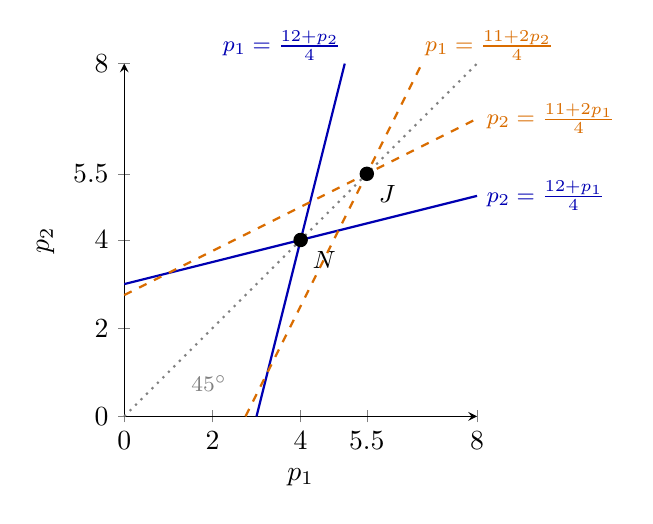
\begin{tikzpicture}
\begin{axis}[
  width=0.5\linewidth, height=0.5\linewidth,
  xmin=0, xmax=8, ymin=0, ymax=8,
  xlabel={$p_1$}, ylabel={$p_2$},
  xtick={0,2,4,5.5,8}, ytick={0,2,4,5.5,8},
  axis lines=left, every axis plot/.append style={thick},
  clip=false]
  \addplot[domain=0:8, samples=2, dotted, gray] {x};
  \addplot[blue!70!black, domain=0:8, samples=2, variable=t] ({(12 + t)/4}, {t});
  \addplot[blue!70!black, domain=0:8, samples=2] {(12 + x)/4};
  \addplot[orange!85!black, dashed, domain=0:8, samples=2, variable=t] ({(11 + 2*t)/4}, {t});
  \addplot[orange!85!black, dashed, domain=0:8, samples=2] {(11 + 2*x)/4};
  \addplot[only marks, mark=*, mark size=2.2pt, black] coordinates {(4,4) (5.5,5.5)};
  \node[anchor=north west, font=\small] at (axis cs:4.05,3.95) {$N$};
  \node[anchor=north west, font=\small] at (axis cs:5.55,5.45) {$J$};
  \node[blue!70!black, anchor=south east, font=\footnotesize, inner sep=1pt] at (axis cs:5.0,8.0) {$p_1 = \frac{12 + p_2}{4}$};
  \node[orange!85!black, anchor=south west, font=\footnotesize, inner sep=1pt] at (axis cs:6.75,8.0) {$p_1 = \frac{11 + 2p_2}{4}$};
  \node[blue!70!black, anchor=west, font=\footnotesize] at (axis cs:8.0,5.0) {$p_2 = \frac{12 + p_1}{4}$};
  \node[orange!85!black, anchor=west, font=\footnotesize] at (axis cs:8.0,6.75) {$p_2 = \frac{11 + 2p_1}{4}$};
  \node[gray, anchor=north west, font=\footnotesize] at (axis cs:1.3,1.15) {$45^\circ$};
\end{axis}
\end{tikzpicture}
\caption{Linear duopoly of \cref{ex:04-linear-duopoly} with $a = 10$, $b = 2$, $d = 1$ and $c = 1$. Solid lines are
the best responses of separate owners, which cross at $N = (4, 4)$. Dashed lines are the first-order loci of a
single owner of both products, each giving the optimal price of one product for a fixed price of the other. They
cross at $J = (5.5, 5.5)$. The dashed loci are not best responses of independent firms. Their slope equals the
diversion ratio $D = \frac{1}{2}$, twice the slope of the separate best responses, because the joint owner
recaptures half of the sales that each product loses.}
\label{fig:04-br-merger}
\end{figure}

\subsection{Worked example: logit demand}\label{sec:04-bertrand-logit}

The logit model gives closed forms for every object in \cref{sec:04-bertrand-matrix}. \Cref{ch:discrete,ch:logit}
derive it from random utility. Here we take the market shares as given. Let market size be one, so quantities
equal shares. Mean utility is $\delta_j = x_j\beta - \alpha p_j + \xi_j$, with observed characteristics $x_j$,
unobserved quality $\xi_j$ and price coefficient $\alpha > 0$. With the mean utility of the outside good
normalized to zero, shares are
\begin{equation*}
s_j(p) = \frac{e^{\delta_j}}{\Phi},
\qquad
s_0(p) = \frac{1}{\Phi},
\qquad
\Phi = 1 + \sum_{k = 1}^{J}e^{\delta_k}.
\end{equation*}
We call $\Phi$ the \emph{logit denominator}.

\casehead{Derivatives}
Changing $p_j$ affects only $e^{\delta_j}$, with $\frac{\partial e^{\delta_j}}{\partial p_j} = -\alpha e^{\delta_j}$,
so also $\frac{\partial\Phi}{\partial p_j} = -\alpha e^{\delta_j}$. The quotient rule gives the own derivative
\begin{align*}
\frac{\partial s_j}{\partial p_j}
&= \frac{(-\alpha e^{\delta_j})\,\Phi - e^{\delta_j}\,(-\alpha e^{\delta_j})}{\Phi^2} \\
&= -\alpha\frac{e^{\delta_j}}{\Phi}\Big(1 - \frac{e^{\delta_j}}{\Phi}\Big)
= -\alpha s_j(1 - s_j).
\end{align*}
For $k \ne j$ the numerator $e^{\delta_k}$ does not depend on $p_j$, so
$\frac{\partial s_k}{\partial p_j} = -\frac{e^{\delta_k}(-\alpha e^{\delta_j})}{\Phi^2} = \alpha s_js_k$. The same
step applies to $s_0 = \frac{1}{\Phi}$. Collecting,
\begin{equation}\label{eq:04-logit-derivs}
\frac{\partial s_j}{\partial p_j} = -\alpha s_j(1 - s_j),
\qquad
\frac{\partial s_k}{\partial p_j} = \alpha s_js_k \quad (k \ne j,\ k \ge 1),
\qquad
\frac{\partial s_0}{\partial p_j} = \alpha s_0s_j.
\end{equation}
These derivatives sum to zero over $k = 0, \dots, J$, as they must. Since $\frac{\partial s_0}{\partial p_j} > 0$,
\cref{prop:04-markup-positive} applies at every price vector. The own and cross elasticities are
\begin{equation*}
\varepsilon_j = \alpha p_j(1 - s_j),
\qquad
\varepsilon_{kj} = \frac{\partial s_k}{\partial p_j}\frac{p_j}{s_k} = \alpha p_js_j \quad \text{for every } k \ne j.
\end{equation*}
A change in $p_j$ moves every other product's share by the same percentage. This is the \emph{independence of
irrelevant alternatives} (IIA), whose consequences \cref{ch:logit} discusses.

\begin{proposition}[Logit markups]\label{prop:04-logit-markup}
Under logit demand with constant marginal costs, every solution of the first-order conditions
\eqref{eq:04-foc-scalar} gives all products of firm $f$ the same markup,
\begin{equation*}
p_j - mc_j = m_f = \frac{1}{\alpha(1 - S_f)}
\quad \text{for all } j \in \mathcal{J}_f,
\qquad
S_f = \sum_{k \in \mathcal{J}_f}s_k.
\end{equation*}
A single-product firm sets $p_j - mc_j = \frac{1}{\alpha(1 - s_j)}$.
\end{proposition}

\begin{proof}
Write the first-order condition for $j \in \mathcal{J}_f$ in shares, $s_j + \sum_{k \in \mathcal{J}_f}m_k\frac{\partial s_k}{\partial p_j} = 0$,
and substitute \eqref{eq:04-logit-derivs}:
\begin{equation*}
s_j - \alpha s_j(1 - s_j)m_j + \sum_{k \in \mathcal{J}_f\setminus\{j\}}\alpha s_js_km_k = 0.
\end{equation*}
Split the second term as $-\alpha s_jm_j + \alpha s_js_jm_j$ and merge $\alpha s_js_jm_j$ into the sum:
\begin{equation*}
s_j - \alpha s_jm_j + \alpha s_j\sum_{k \in \mathcal{J}_f}s_km_k = 0.
\end{equation*}
Divide by $\alpha s_j > 0$:
\begin{equation*}
m_j = \frac{1}{\alpha} + \sum_{k \in \mathcal{J}_f}s_km_k.
\end{equation*}
The right side is the same for every $j \in \mathcal{J}_f$, so all of the firm's products share one markup $m_f$.
Substituting $m_k = m_f$ gives $m_f = \frac{1}{\alpha} + S_fm_f$. Since $S_f \le 1 - s_0 < 1$, we can solve:
$m_f = \frac{1}{\alpha(1 - S_f)}$. A single-product firm has $S_f = s_j$.
\end{proof}

The proposition characterizes markups without giving them in closed form, because $S_f$ depends on prices. It
still has several sharp implications. Markups are bounded below by $\frac{1}{\alpha}$, whatever the number of
competitors. They depend on the firm only through its combined share. Product quality and cost affect markups
only by changing shares. Within a firm, dollar markups are equal, so a firm's high-cost products carry lower
percentage margins, $\frac{m_f}{p_j} = \frac{1}{\alpha p_j(1 - S_f)}$. Finally, a firm with a large combined share
sets high markups on all its products, including those with tiny shares.

As an illustration, suppose one firm owns products 1 and 2 with shares $s_1$ and $s_2$. It sets the markup
$\frac{1}{\alpha(1 - s_1 - s_2)}$ on both. If the products had separate owners, their markups would be
$\frac{1}{\alpha(1 - s_1)}$ and $\frac{1}{\alpha(1 - s_2)}$. Joint ownership raises the markup of the smaller
product by more. Under logit, the diversion ratio from product $k$ to product $j$ is $\frac{s_j}{1 - s_k}$
(\cref{sec:04-diversion-systems}). Diversion from the small product to the large one is therefore the larger of the
two, so joint ownership recaptures a larger fraction of the small product's lost sales.

\casehead{The best response in closed form}
For a single-product firm the first-order condition $\alpha m_j(1 - s_j) = 1$ is implicit, because $s_j$ depends
on $p_j$. It can nevertheless be solved explicitly. Define the mean utility of product $j$ at marginal-cost
pricing and the logit denominator without product $j$,
\begin{equation*}
v_j = x_j\beta + \xi_j - \alpha\,mc_j,
\qquad
\Phi_{-j} = 1 + \sum_{l \ne j}e^{\delta_l}.
\end{equation*}
Then $\delta_j = v_j - \alpha m_j$, and $\Phi_{-j}$ depends only on rivals' prices. The share and its complement
are
\begin{equation*}
s_j = \frac{e^{\delta_j}}{\Phi_{-j} + e^{\delta_j}},
\qquad
1 - s_j = \frac{\Phi_{-j}}{\Phi_{-j} + e^{\delta_j}}.
\end{equation*}
Substitute the complement into the first-order condition and multiply by $\Phi_{-j} + e^{\delta_j}$:
\begin{align*}
\alpha m_j\Phi_{-j} &= \Phi_{-j} + e^{\delta_j} \\
(\alpha m_j - 1)\Phi_{-j} &= e^{v_j - \alpha m_j}.
\end{align*}
Multiply both sides by $\frac{e^{\alpha m_j - 1}}{\Phi_{-j}}$:
\begin{equation*}
(\alpha m_j - 1)\,e^{\alpha m_j - 1} = \frac{e^{v_j - 1}}{\Phi_{-j}}.
\end{equation*}
The \emph{Lambert W function} $W(z)$ solves $W(z)e^{W(z)} = z$ \citep{CorlessEtAl1996}. For $z > 0$ the equation
$ye^y = z$ has exactly one real root, which is positive. Indeed $ye^y \le 0$ for $y \le 0$, while $ye^y$ rises
strictly from 0 to infinity on $y > 0$. Setting $y = \alpha m_j - 1$ gives the best response
\begin{equation}\label{eq:04-logit-br}
BR_j(p_{-j}) = mc_j + \frac{1}{\alpha}\Big[1 + W\Big(\frac{e^{v_j - 1}}{\Phi_{-j}}\Big)\Big].
\end{equation}
The formula shows three properties at a glance. The best-response markup exceeds $\frac{1}{\alpha}$ because
$W(z) > 0$. It rises with the product's quality net of cost, $v_j$. And it rises with every rival price, because
a higher $p_l$ lowers $\Phi_{-j}$ and $W$ is increasing. Logit prices are strategic complements.

The stationary point in \eqref{eq:04-logit-br} is the global maximizer of $\pi_j = m_js_j$. The derivative of
profit factors as
\begin{equation*}
\frac{\partial\pi_j}{\partial p_j} = s_j + m_j\frac{\partial s_j}{\partial p_j} = s_j\,g(p_j),
\qquad
g(p_j) = 1 - \alpha(p_j - mc_j)\big(1 - s_j(p_j)\big).
\end{equation*}
If $p_j \le mc_j$, then $g(p_j) \ge 1$ and profit is increasing. If $p_j > mc_j$, both $\alpha(p_j - mc_j)$ and
$1 - s_j(p_j)$ are positive and strictly increasing in $p_j$, so $g$ is strictly decreasing. As
$p_j \to \infty$, $g(p_j) \to -\infty$. Hence $g$ crosses zero exactly once, from above. Profit rises before the
crossing and falls after it, so the crossing is the unique global maximizer.

The multi-product analogue follows the same steps. By \cref{prop:04-logit-markup}, a stationary point of firm
$f$'s problem has a common markup $m_f$, so $e^{\delta_k} = e^{v_k - \alpha m_f}$ for $k \in \mathcal{J}_f$. Let
$E_f = \sum_{k \in \mathcal{J}_f}e^{v_k}$ and $\Phi_{-f} = 1 + \sum_{l \notin \mathcal{J}_f}e^{\delta_l}$. The
firm's combined share is
\begin{equation*}
S_f = \frac{E_fe^{-\alpha m_f}}{\Phi_{-f} + E_fe^{-\alpha m_f}}.
\end{equation*}
Repeating the algebra above with $E_f$ in place of $e^{v_j}$ and $S_f$ in place of $s_j$ gives
\begin{equation}\label{eq:04-logit-br-multi}
m_f^{BR}(p_{-\mathcal{J}_f}) = \frac{1}{\alpha}\Big[1 + W\Big(\frac{E_fe^{-1}}{\Phi_{-f}}\Big)\Big],
\qquad
p_k = mc_k + m_f^{BR} \ \text{ for } k \in \mathcal{J}_f.
\end{equation}
Showing that this stationary point is the firm's global optimum takes one more step. The firm's problem reduces to
the choice of a common markup, and the single-crossing argument then applies to $S_f$ in place of $s_j$. Steps 1
and 2 of the proof of \cref{thm:04-logit-unique} give the details, and \cref{sec:04-exercises} asks for the
algebra behind \eqref{eq:04-logit-br-multi}.

\subsection{A numerical illustration: 25 logit products}\label{sec:04-bertrand-logit25}

We now compute equilibria in a simulated market. The market reappears in \cref{sec:04-existence}, where we check
uniqueness, and as a worked problem in \cref{app:problems}.

\begin{example}[A 25-product logit market]\label{ex:04-logit25}
There are $J = 25$ products and market size one. Each product has three observed characteristics: a constant, a
continuous characteristic and a binary one, $x_j = (1, x_{j2}, x_{j3})$. It also has unobserved quality $\xi_j$ and
a cost shock $\omega_j$. Demand is logit with $\beta = (0.1, 0.25, 0.1)$ and $\alpha = 2$. Marginal cost is
$mc_j = x_j\gamma + \omega_j$ with $\gamma = (0.2, 0.25, 0.3)$, and it ranges from 0.164 to 1.236. All primitives
are common knowledge, and firms set prices simultaneously. We compare two ownership structures.
\begin{itemize}
  \item[(S)] Every product has its own owner, so $\Omega = I_{25}$.
  \item[(M)] Five owners, labeled 0 to 4, hold 3, 3, 6, 6 and 7 products.
\end{itemize}
Products are numbered 0 to 24 and owners 0 to 4, as in the data set of \cref{app:problems}. Here the label 0 names
an inside product, and $s_0$ still denotes the share of the outside good.
In (S) the first-order conditions are $s_j + (p_j - mc_j)\frac{\partial s_j}{\partial p_j} = 0$ for all $j$. In
(M) they are $s + (\Omega \odot \Delta^{s\top})(p - mc) = 0$ with the owners' $\Omega$. A Nash equilibrium is a
price vector at which no owner can raise its profit by changing its own prices, which is a fixed point of the
best-response map.
\end{example}

\begin{remark}[Computing the equilibrium]\label{rem:04-logit25-algorithm}
We compute each equilibrium by best-response iteration.
\begin{enumerate}
  \item Start from $p^{(0)} = mc + \frac{1}{\alpha}$, the lower bound on logit markups.
  \item Given $p^{(n)}$, compute for every owner $f$ the quantities $E_f$ and $\Phi_{-f}(p^{(n)})$, the markup
  $m_f$ from \eqref{eq:04-logit-br-multi}, and set $p^{(n+1)}_k = mc_k + m_f$ for $k \in \mathcal{J}_f$. In (S)
  every owner has one product and the step is \eqref{eq:04-logit-br}.
  \item Stop when $\|p^{(n+1)} - p^{(n)}\|_\infty < 10^{-12}$. Otherwise return to step 2.
  \item Check that the first-order residuals $s + (\Omega \odot \Delta^{s\top})(p - mc)$ vanish and that each
  owner's markup equals $\frac{1}{\alpha(1 - S_f)}$.
\end{enumerate}
The iteration converges in 10 steps in (S) and 15 steps in (M). As a cross-check we also iterate on the markup
equation, $p \leftarrow mc - (\Omega \odot \Delta^s(p)^\top)^{-1}s(p)$, which converges in 14 and 30 steps to the
same prices (largest difference $1.4 \times 10^{-13}$). The largest first-order residual is below
$2 \times 10^{-14}$. Markup iteration is simple and fast here, but it is not guaranteed to converge in general
(\cref{sec:04-counterfactuals}).
\end{remark}

\Cref{tab:04-logit25} reports the results by owner, and \cref{fig:04-logit25-markups} shows every product's
markup. In (S) each product is priced by a separate firm, and the owner rows aggregate those products for
comparison with (M). Consumer surplus is measured by $\frac{1}{\alpha}\ln\Phi$, the logit expected maximum utility
in money units (\cref{ch:logit}). We measure it relative to a market in which only the outside good is available,
where $\Phi = 1$. Its level is then the surplus that consumers get from the inside goods, so percentage changes are
meaningful.

\begin{table}[htbp]
\centering
\caption{Bertrand-Nash equilibrium in the 25-product logit market}
\label{tab:04-logit25}
\footnotesize
\begin{tabular}{@{}lccccccc@{}}
\toprule
 & & \multicolumn{2}{c}{Combined share $S_f$ (\%)} & \multicolumn{2}{c}{Markup} & \multicolumn{2}{c}{Profit $\times 100$} \\
\cmidrule(lr){3-4}\cmidrule(lr){5-6}\cmidrule(l){7-8}
Owner & Products & (S) & (M) & (S) & (M) & (S) & (M) \\
\midrule
\multicolumn{8}{@{}l}{\textit{Panel A. Owners}} \\
0 & 3 & 18.32 & 18.87 & 0.552 & 0.616 & 10.112 & 11.632 \\
1 & 3 & 4.12 & 4.67 & 0.508 & 0.524 & 2.094 & 2.449 \\
2 & 6 & 13.27 & 13.68 & 0.516 & 0.579 & 6.841 & 7.925 \\
3 & 6 & 22.62 & 21.40 & 0.529 & 0.636 & 11.971 & 13.616 \\
4 & 7 & 28.00 & 25.36 & 0.541 & 0.670 & 15.145 & 16.989 \\
\midrule
\multicolumn{8}{@{}l}{\textit{Panel B. Market}} \\
\multicolumn{4}{@{}l}{Outside share $s_0$} & 0.1367 & 0.1601 & & \\
\multicolumn{4}{@{}l}{Logit denominator $\Phi^* = \frac{1}{s_0}$} & 7.314 & 6.246 & & \\
\multicolumn{4}{@{}l}{Consumer surplus $\frac{1}{\alpha}\ln\Phi^*$} & 0.9949 & 0.9159 & & \\
\multicolumn{4}{@{}l}{Total profit} & 0.4616 & 0.5261 & & \\
\multicolumn{4}{@{}l}{Total surplus (consumer surplus plus profit)} & 1.4565 & 1.4421 & & \\
\multicolumn{4}{@{}l}{Share-weighted mean price} & 1.2599 & 1.3553 & & \\
\bottomrule
\end{tabular}

\vspace{3pt}
\begin{minipage}{0.97\textwidth}
\footnotesize Notes: (S) single-product firms, (M) five multi-product owners. In column (S) the owner rows add
up shares and profits of products that are priced independently, and the markup is the share-weighted mean
over the owner's products. In column (M) every product of an owner carries the same markup
$\frac{1}{\alpha(1 - S_f)}$. Market size is one, so profits and consumer surplus are per consumer. Computed with
\texttt{figures/ch04/src/logit25.py}.
\end{minipage}
\end{table}

\begin{figure}[htbp]
\centering
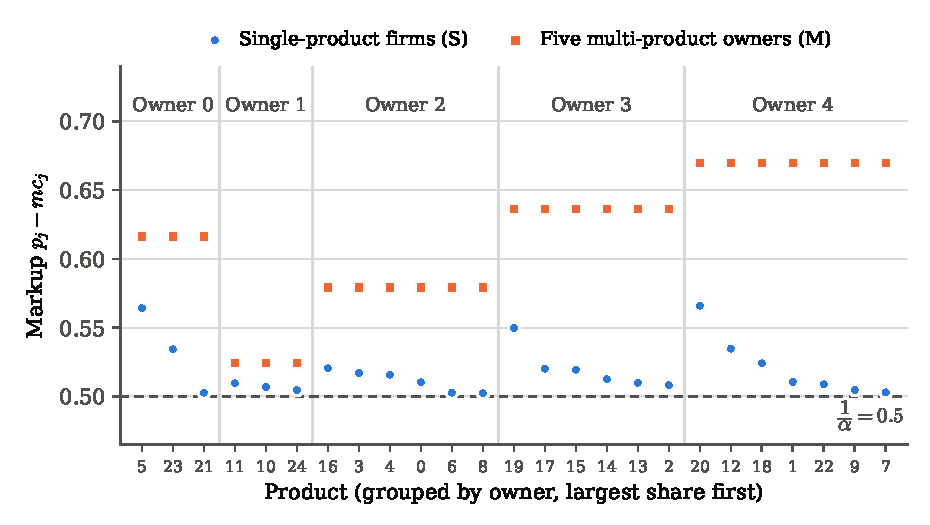
\includegraphics[width=\linewidth]{figures/ch04/logit25_markups.pdf}
\caption{Equilibrium markups $p_j - mc_j$ in the 25-product logit market. Circles show single-product firms (S),
squares show the five multi-product owners (M). Products are grouped by owner and sorted by share. Under (S)
markups are close to the floor $\frac{1}{\alpha} = 0.5$ and rise with the product's own share. Under (M) all
products of an owner share the markup $\frac{1}{\alpha(1 - S_f)}$.}
\label{fig:04-logit25-markups}
\end{figure}

The results illustrate the theory of this section in five ways.

First, single-product markups lie between 0.502 and 0.566, close to the floor $\frac{1}{\alpha} = 0.5$. Each
product has a small share, so $\frac{1}{\alpha(1 - s_j)}$ barely exceeds $\frac{1}{\alpha}$. The largest markups
belong to the products with the largest shares, products 20 and 5, whose shares are 11.7 and 11.4 percent.

Second, multi-product ownership raises every owner's markup to $\frac{1}{\alpha(1 - S_f)}$. The common markups range
from 0.524 for owner 1, whose products have a combined share near 5 percent, to 0.670 for owner 4, whose
combined share is about 25 percent. A product with a share of half a percent, such as product 7, carries the same
markup as owner 4's largest product. Its price rises the most, by 0.167.

Third, every price rises, by amounts from 0.015 (product 11) to 0.167 (product 7). Two forces combine. Each owner
internalizes cannibalization among its own products, and prices are strategic complements, so each owner also
responds to the higher prices of the others. To isolate the second force, we recomputed the equilibrium with only
owner 4 consolidating its seven products and all other products independent. Owner 4's prices rise by 0.089 to
0.152, and rivals' prices rise by 0.0001 to 0.0040 through strategic complementarity. In that exercise rivals'
combined profit rises from 0.3102 to 0.3296, while owner 4's profit rises only from 0.1515 to 0.1553. The
non-consolidating firms gain more than the firm that consolidates.

Fourth, shares move away from the owners that raise prices most. The two largest owners lose share, owner 4
from 28.00 to 25.36 percent and owner 3 from 22.62 to 21.40 percent. The three smaller owners gain. Fifteen of the
25 products lose share, and the outside share rises from 0.137 to 0.160.

Fifth, total profit rises by about 14 percent, from 0.4616 to 0.5261. Consumer surplus falls by 0.079, or 7.9
percent, and total surplus falls from 1.4565 to 1.4421. In equilibrium the logit denominator equals
$\frac{1}{s_0}$, which falls from 7.314 to 6.246. \Cref{sec:04-existence} shows that this aggregate pins down
the whole equilibrium. It uses this to prove that the logit equilibrium is unique for any ownership structure
\citep{KonovalovSandor2010,NockeSchutz2018}, and \cref{ex:04-logit25-unique} confirms numerically that the two
equilibria in \cref{tab:04-logit25} are the only ones.
